\documentclass[UTF8,a4paper,12pt]{ctexbook} 

\usepackage{graphicx}%学习插入图
\usepackage{verbatim}%学习注释多行
\usepackage{booktabs}%表格
\usepackage{geometry}%图片
\usepackage{amsmath}
\usepackage{amssymb}
\usepackage{listings}%代码
\usepackage{xcolor}  %颜色
\usepackage{enumitem}%列表格式
\usepackage{tcolorbox}
\usepackage{algorithm}  %format of the algorithm
\usepackage{algorithmic}%format of the algorithm
\usepackage{multirow}   %multirow for format of table
\usepackage{tabularx} 	%表格排版格式控制
\usepackage{array}	%表格排版格式控制
\usepackage{hyperref} %超链接 \url{URL}
\usepackage{tikz}
\usepackage{dirtree}

\CTEXsetup[format+={\flushleft}]{section}

%%%% 设置图片目录
\graphicspath{{figure/}}

%%%% 段落首行缩进两个字 %%%%
\makeatletter
\let\@afterindentfalse\@afterindenttrue
\@afterindenttrue
\makeatother
\setlength{\parindent}{2em}  %中文缩进两个汉字位

%%%% 下面的命令重定义页面边距,使其符合中文刊物习惯 %%%%
\addtolength{\topmargin}{-54pt}
\setlength{\oddsidemargin}{0.63cm}  % 3.17cm - 1 inch
\setlength{\evensidemargin}{\oddsidemargin}
\setlength{\textwidth}{14.66cm}
\setlength{\textheight}{24.00cm}    % 24.62

%%%% 下面的命令设置行间距与段落间距 %%%%
\linespread{1.4}
\setlength{\parskip}{0.5\baselineskip}
\geometry{left=1.6cm,right=1.8cm,top=2cm,bottom=1.7cm} %设置文章宽度
\pagestyle{plain} 		  %设置页面布局

%代码效果定义
\definecolor{mygreen}{rgb}{0,0.6,0}
\definecolor{mygray}{rgb}{0.5,0.5,0.5}
\definecolor{mymauve}{rgb}{0.58,0,0.82}
\lstset{ %
	backgroundcolor=\color{white},   % choose the background color
	basicstyle=\footnotesize\ttfamily,      % size of fonts used for the code
	%stringstyle=\color{codepurple},
	%basicstyle=\footnotesize,
	%breakatwhitespace=false,         
	%breaklines=true,                 
	%captionpos=b,                    
	%keepspaces=true,                 
	%numbers=left,                    
	%numbersep=5pt,                  
	%showspaces=false,                
	%showstringspaces=false,
	%showtabs=false,        
	columns=fullflexible,
	breaklines=true,                 % automatic line breaking only at whitespace
	captionpos=b,                    % sets the caption-position to bottom
	tabsize=4,
	commentstyle=\color{mygreen},    % comment style
	escapeinside={\%*}{*)},          % if you want to add LaTeX within your code
	keywordstyle=\color{blue},       % keyword style
	stringstyle=\color{mymauve}\ttfamily,     % string literal style
	frame=single,
	xleftmargin = .05\textwidth,
	rulesepcolor=\color{red!20!green!20!blue!20},
	% identifierstyle=\color{red},
	language=c++,
}
 \author{\kaishu 郑华}
 \title{\heiti Shader 笔记}
 
\begin{document}          %正文排版开始
 	\maketitle
	\tableofcontents 

\chapter{着色器}
	
	
	
				
\chapter{基础概念}
	
	\section{Draw Call}	

	\section{Shader}
		\paragraph{可以干啥}
		
			屏幕特效实现下雪
			
			静态纹理的动态化,如波浪、水流等
			
			光照的应用
			
			投影
	
		\paragraph{常用的Shader 语言}
				\begin{itemize}
					\item OpenGL GLSL(opengGL Shader Language) SGI公司开发的跨平台。
					\item DirectX  HLSL(High Level Shader Language) 微软
					\item \textbf{->CG} 微软和英伟达联合开发的跨平台, 基于C语言。
					\item \textbf{->Shader Lab} Unity3D 自己的shader 语言。
				\end{itemize}
		
		\paragraph{矩阵变换}
				\verb|Unity 3D |矩阵一般是\textbf{左乘}。在\verb|Shader| 中的前缀为\verb|UNITY_MATRIX_|
				
				\begin{enumerate}[itemindent = 1em]
					\item \verb|M|: 将物体坐标系变换到世界坐标系
					\item \verb|V|: 将世界坐标系 变换到 相机坐标系
					\item \verb|P|: 将3D坐标系 转换成 2维屏幕坐标系
				\end{enumerate}
				
				当然在脚本中也可以完成类似功能,如
			
			\verb|Transform.parent.localToWorldMatrix.MultiplyPoint(tranform.localPosition)|.
	\section{Shader 版本}
			Shader 1.0(DirectX8.0)、
			Shader 2.0(DirectX9.0b)、
			Shader 3.0(DirectX9.0c)、
			Shader 4.0(DirectX10)、
			Shader 4.1(DirectX10.1)
			和Shader 5(DirectX11)。
	
			\begin{figure}[H]
				\centering
				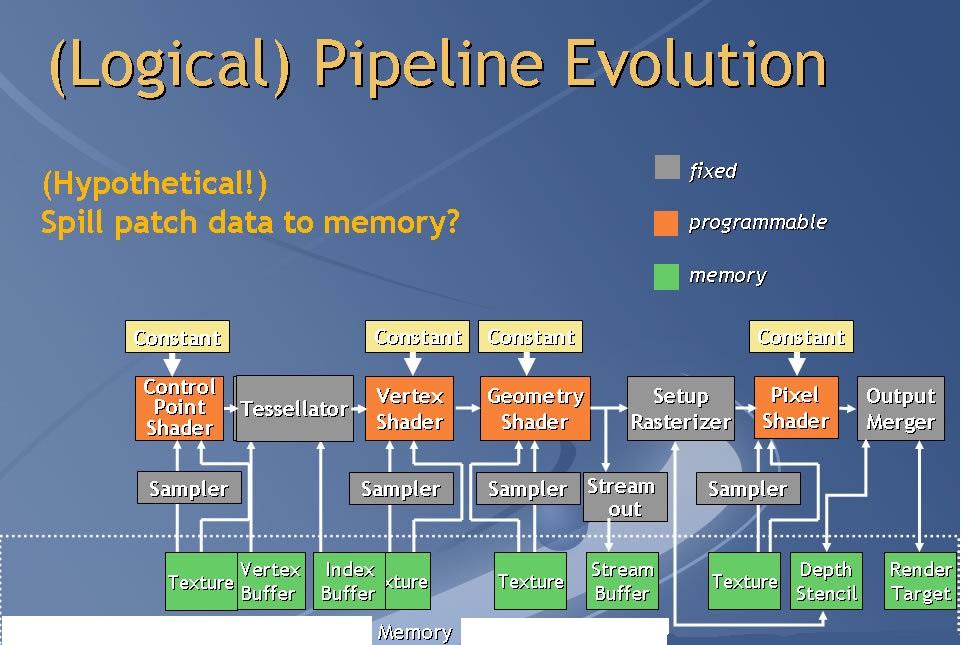
\includegraphics[scale=0.71]{ShaderArc}
				\caption{shader  通用架构}
			\end{figure}
			
			
	\section{结构}
		\begin{figure}[H]
			\centering
			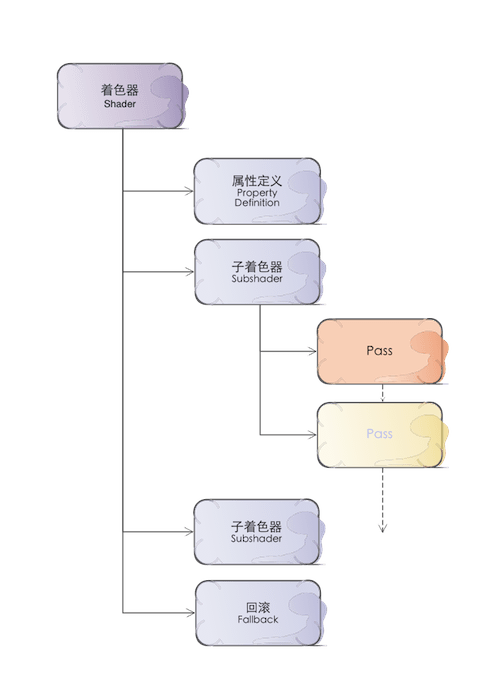
\includegraphics[scale=0.8]{arch}
			\caption{着色器结构}
		\end{figure}
		
		\begin{itemize}
			\item \textbf{属性定义(Property Definition)}:定义Shader的输入,并且绑定到编辑器上。
			\item \textbf{子着色器(SubShader)}:\underline{一个Shader可以有多个子着色器。}这些子着色器互不相干且\textbf{只有一个会在最终的平台运行}。\textit{编写多个的目的是解决兼容性问题。Unity会自己选择兼容终端平台的Shader运行}。
			\item \textbf{回滚(Fallback)}:如果子着色器在终端平台上都无法运行,那么使用Fallback指定的备用Shader,\textbf{俗称备胎}。
			\item \textbf{Pass}:\textit{一个Pass就是一次绘制}。\textbf{对于表面着色器,只能有一个Pass},所以不存在Pass节。\textbf{顶点片段着色器可以有多个Pass。}多次Pass可以实现很多特殊效果,例如当人物被环境遮挡时还可以看到人物轮廓就可以用多Pass来实现。
			\item \textbf{Cg代码}:每个Pass中都可以包含自定义的Cg代码,\textbf{从CGPROGRAM开始到ENDCG结束}。
		\end{itemize}
		
		\paragraph{常用语义}
			POSITION\textbf{语义}等相当于告诉渲染引擎,这个变量是代表什么含义。
			
			\begin{itemize}
				\item \verb|POSITION| 获取模型顶点信息。
				\item \verb|NORMAL| 获取法线信息。
				\item \verb|TEXCOORD n| 第(n)张贴图的uv坐标
				\item \verb|COLOR n| 第n个定点色。\verb|float4|
				\item \verb|TANGENT| 获取切线信息
				\item \verb|SV_POSITION| 表示经过MVP 矩阵已经转化到屏幕坐标的位置
				\item \verb|SV_TARGET| 输出到哪个Render Target 上
 			\end{itemize}
		
		\paragraph{常用坐标系}
			\begin{itemize}
				\item \verb|模型坐标系|:也叫物体坐标系,3D建模的时候每个模型都是在自己的坐标系下建立的,如果一个人物模型脚底是(0,0,0) 点的话它的身上其它点的坐标都是相对脚底这个原点的。 
				\item \verb|世界坐标系|:我们场景是一个世界,有自己的原点,模型放置到场景中后模型上的每个顶点就有了一个新的世界坐标。这个坐标可以通过模型矩阵×模型上顶点的模型坐标得到。 
				\item \verb|视图坐标系|:又叫观察坐标系,是以观察者(相机)为原点的坐标系。场景中的物体只有被相机观察到才会绘制到屏幕上,相机可以设置视口大小和裁剪平面来控制可视范围,这些都是相对相机来说的,所以需要把世界坐标转换到视图坐标系来方便处理。 
				\item \verb|投影坐标系|:场景是3D的,但是最终绘制到屏幕上是2D,投影坐标系完成这个降维的工作,投影变换后3D的坐标就变成2D的坐标了。投影有平行投影和透视投影两种,可以在Unity的相机上设置。 
				\item \verb|屏幕坐标系|: 最终绘制到屏幕上的坐标。屏幕的左下角为原点。
			\end{itemize}

		\paragraph{常用矩阵表示}
			\begin{itemize}
				\item \verb|UNITY_MATRIX_MVP|:当前模型 -> 视图 -> 投影矩阵。(注:模型矩阵为 本地->世界)
				\item \verb|UNITY_MATRIX_MV|:当前模型 -> 视图矩阵
				\item \verb|UNITY_MATRIX_V|:当前视图矩阵
				\item \verb|UNITY_MATRIX_P|:当前投影矩阵
				\item \verb|UNITY_MATRIX_VP|:当前视图 -> 投影矩阵
				\item \verb|UNITY_MATRIX_T_MV|:转置模型 -> 视图矩阵
				\item \verb|UNITY_MATRIX_IT_MV|:逆转置模型 -> 视矩阵, 用于将法线从\verb|ObjectSpace|旋转到\verb|WorldSpace|。为什么法线变化不能和位置变换一样用\verb|UNITY_MATRIX_MV|呢?一是因为法线是3维的向量而- \verb|UNITY_MATRIX_MV|是一个4x4矩阵,二是因为法线是向量,我们只希望对它旋转,但是在进行空间变换的时候,如果发生非等比缩放,方向会发生偏移。
				\item \verb|UNITY_MATRIX_TEXTURE0 |to \verb|UNITY_MATRIX_TEXTURE3|:纹理变换矩阵
			\end{itemize}
			
	\section{Shader2.0}
		可以实现编程。
		
		\url{https://www.cnblogs.com/lixiang-share/p/5025662.html}
		
		\paragraph{大概流程}
			\dirtree{%
				.1 .
				.2 MeshRender 将CPU数据传入至GPU .
				.3 然后传递给顶点着色器 .
				.4 顶点着色器处理完成后,将自己的输出数据传递给 片段着色器处理 .
			}

		
		\paragraph{定义顶点着色器入口函数}
			\verb|#pragma vertex _vertexFunctionName |
			
		\paragraph{定义片段着色器入口函数}
			\verb|#pragma fragment _fragmentFunctionName |

		\paragraph{定义平面着色器入口函数}
			\verb|#pragma surface _surfaceFunctionName |
			
		
		
			
	\section{材质、贴图、纹理}
			材质 Material包含贴图 Map,贴图包含纹理 Texture。
			
			\paragraph{纹理}\verb|->|
			
				是最基本的数据输入单位,游戏领域基本上都用的是位图。常见格式有PNG,TGA,BMP,TIFF此外还有程序化生成的纹理 Procedural Texture。 
				在内存中通常表示为二维像素数组。
				
			\paragraph{贴图}\verb|->|
			
				英语 Map 其实包含了另一层含义就是“映射”。其功能就是\underline{把}\textbf{纹理}通过 \verb|UV 坐标| \underline{映射}到 \textit{3D 物体表面}。
				
				\textbf{贴图}\textit{包含了}\textbf{除了纹理以外其他很多信息},比方说 \textbf{UV 坐标}、\textbf{贴图输入输出控制}等等。 
				一张图便能说明其之间的关系 
				\begin{figure}[H]
					\centering
					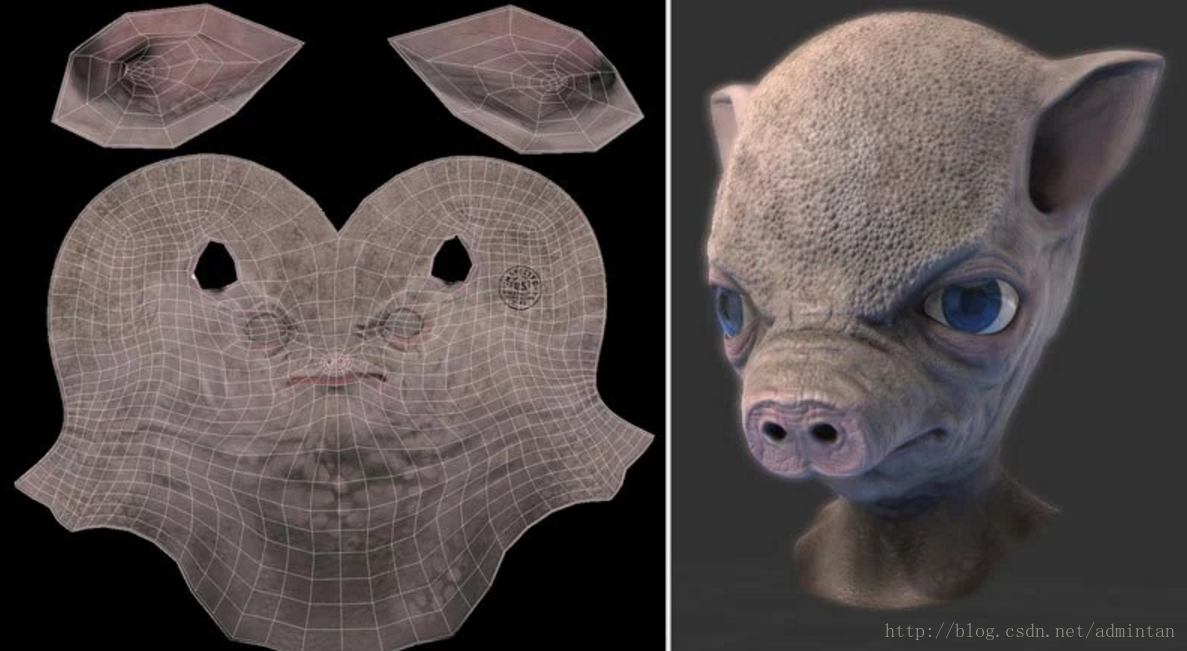
\includegraphics[scale=0.57]{Texture}
					\caption{纹理与贴图}
				\end{figure}
				
			\paragraph{材质}\verb|->|
			
				本质就是一个\textbf{数据集},主要功能就是\textbf{给渲染器}\textit{提供数据和光照算法}。
				
				\textbf{贴图}就是其中\textbf{数据的一部分},根据用途不同,贴图也会被分成不同的类型,比方说 \verb|Diffuse Map|,\verb|Specular Map|,\verb|Normal Map| 和 \verb|Gloss Map| 等等。
				
				\textbf{另外一个重要部分}就是\textbf{光照模型 Shader} ,用以实现不同的渲染效果。 贴图种类繁多:我做个不完全总结
				
				\subparagraph{Diffuse Map}
					漫反射贴图/也被称作反照率贴图albedo map, 存储了物体相应部分漫反射颜色
					
				\subparagraph{Normal Map}
					法线贴图 本质上存储的是被RGB值编码的法向量 表现凹凸,\textbf{比如一些凹凸不平的表面,光影在表面产生实时变化,常用来低精度多边形表现高精度多边形细节}, \textbf{比如在高多边形下生成normal map在匹配给低多边形模型 是一种常见的降低性能要求的做法}
					
					\begin{figure}[H]
						\centering
						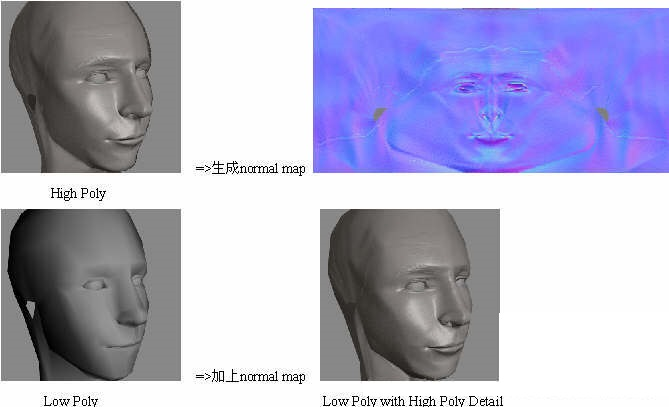
\includegraphics[scale=0.8]{normalMap}
						\caption{法线贴图演示}
					\end{figure}
					
					建议参考:\url{https://blog.csdn.net/cywater2000/article/details/749341#comments}
					
					常规来说就是\textbf{光向量}和\textbf{法向量}的\textbf{点积}\textit{来确定明暗以表现凹凸质感},也就是把法线存在纹理中。
				\subparagraph{Specular Map}
					高光贴图 表现质感 高光区域大小可真实反映材质区别
					
				\subparagraph{Gloss Map}
					光泽贴图,每个纹理元素上描述光泽程度
					
			总体上说 他们都是要被shader加工的原材料.
	
	\section{光照模型}
		参考:\url{https://blog.csdn.net/admintan/article/details/53913624}
		
		\subsection{Phone 光照模型}
			真实世界中的光照效果抽象为三种独立的光照效果的叠加。
				$$Color = Ambient + Diffuse + Specular$$
			
			\paragraph{环境光-Ambient}
				此为模拟环境中的整体光照水平,是间接反射光的粗略估计,间接反射的光使阴影部分不会变成全黑 关于环境光还有个事实,1某个可以独立分析的局部场合的环境光强和能够进入这个地方的光的强度有关。 
					
					$$Ambient = K_a * GlobalAmbient $$
					
			\paragraph{漫反射光-Diffuse}
				模拟直接光源在表面均匀的向各个方向反射,能够逼近真实光源照射到哑光表面的反射。比如在阳光下,由于路面粗糙的性质,我们发现从任意一个角度观察路面,亮度都是差不多。 
				
					$$Diffuse = K_d * lightColor * dot(L,N) $$
			\paragraph{镜面反射光-Specular}
				模拟在光滑表面会看到的光亮高光。会出现在光源的直接反射方向。镜子、金属等表面光亮的物体会有镜面反射光。镜面反射光同时与物体表面朝向、光线方向、视点位置有关。如图:
					\begin{figure}[H]
						\centering
						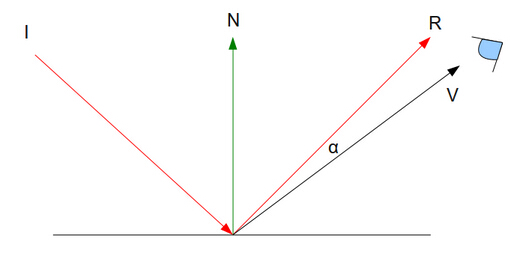
\includegraphics[scale=0.8]{Specular}
						\caption{高光演示}
					\end{figure}
				
				$I$是入射光,$N$是表面法线,$R$是反射光线,$V$是从物体上的目标观察点指向视点的向量,$a$是$V$和$R$的夹角。
				
				我们可以判断出一个规律,夹角$a$越小,即视线与反射方向的偏离越小,则目标点的光强越大,计算公式为:
					
					$$Specular = K_s * lightColor * (dot(V,R))^{shininess}$$ 
				
					\begin{itemize}
						\item Ks为物体对于反射光线的衰减系数
						\item Shininess为高光指数,高光指数反映了物体表面的光泽程度。
						\begin{itemize}
							\item Shininess越大,反射光越集中,当偏离反射方向时,光线衰减的越厉害,只有当视线方向与反射光线方向非常接近时才能看到镜面反射的高光现象,此时,镜面反射光将会在反射方向附近形成亮且小的光斑;
							\item Shininess 越小,表示物体越粗糙,反射光分散,观察到的光斑区域小,强度弱。
						\end{itemize}
					\end{itemize}
			
			\paragraph{总结}
				至于更多的光照模型结合了更多的物理光学等信息 在模拟单种材质例如塑料 合金 石膏陶瓷等等上要好于Phone式模型的效果 但是基本上属于Phone式模型的扩充
					
	\section{参考}
			入门参考网址:\url{https://blog.csdn.net/ring0hx/article/details/46440037}	
			
\chapter{流水线}
	The Main Function of the pipeline is \textbf{to Generate} or \textbf{Render}, \textbf{a two-dimensional Image}, \textit{given a virtual camera, three-dimensional objects, light sources, and more}.
	
	
	\section{渲染流水线}
		\begin{tikzpicture}\\
			\def \width {16};
			\def \height {3};
			\def \leftBottom {(0, 0)};
			\def \rightTop {(\width, \height)};
			
			%基底
			\draw[ultra thick] \leftBottom rectangle \rightTop;
			
			%应用阶段
			\draw[fill=blue,ultra thick] (\width/5*0,\height/3*1) rectangle (\width/5*1, \height/3*2);
			\node[yellow, ultra thick,scale = 1.5] at (\width/5*0.5,\height/2) {\textbf{应用阶段}};
			\draw[->,line width =.2cm] (\width/5, \height/2) -- (\width/5*2, \height/2);
			
			%几何阶段
			\draw[fill=red,ultra thick] (\width/5*2,\height/3*1) rectangle (\width/5*3, \height/3*2);
			\node[yellow, ultra thick,scale = 1.5] at (\width/5*2.5,\height/2) {\textbf{几何阶段}};
			\draw[->,line width =.2cm] (\width/5*3, \height/2) -- (\width/5*4, \height/2);

			
			\draw[fill=red,ultra thick] (\width/5*4,\height/3*1) rectangle (\width, \height/3*2);
			\node[yellow, ultra thick,scale = 1.5] at (\width/5*4.5,\height/2) {\textbf{光栅化阶段}};
		\end{tikzpicture}
		
		具体细节可以参考\textbf{图形学原理笔记}。
		
		\paragraph{应用阶段}
			这个阶段主要由应用主导的,通常由CPU 负责实现。即这个阶段开发者拥有绝对控制权。
			\begin{enumerate}
				\item \textbf{准备场景数据}
					\begin{itemize}
						\item 模型、贴图
						\item 相对位置(世界变换)
						\item 摄像机
						\item 视椎体(投影变换)
						\item 光源等。
					\end{itemize}
				\item \textbf{粗粒度剔除工作}
					\begin{itemize}
						\item 将不在场景中的物体剔除出去。
					\end{itemize}
				\item \textbf{设置好每个模型的渲染状态}
					\begin{itemize}
						\item 使用的材质
						\item 使用的纹理
						\item 使用的Shader
					\end{itemize}
			\end{enumerate}
		
		\paragraph{几何阶段}
			这个阶段决定需要绘制的图元是什么,怎么绘制他们,在哪里绘制他们,这一阶段一般在GPU上。
			
			\begin{enumerate}
				\item \textbf{顶点着色器}
					\begin{itemize}
						\item 计算顶点的颜色
						\item 将物体坐标系 转换到 相机坐标系(相机变换)
					\end{itemize}
				\item 裁剪
				\item 屏幕映射
			\end{enumerate}
		
		\paragraph{光栅化阶段}
			将\textbf{顶点}\underline{转换为}\textbf{像素}。
			
			\begin{enumerate}
				\item 三角形设置
				\item 三角形遍历
					\begin{itemize}
						\item 输入:顶点
						\item 插值:将适当地方填充
						\item 输出:像素
					\end{itemize}
				\item \textbf{片段着色器}
					\begin{itemize}
						\item 输入:像素(RGBA 4通道组成)
						\item \textbf{纹理采样}: 从纹理像素 赋值给 像素,\textbf{覆盖}以前默认像素(三角形遍历阶段插值的像素颜色)颜色值。
						\item 像素跟\textbf{灯光计算}。
					\end{itemize}					
				\item \textbf{三大测试}
					\begin{itemize}
						\item alpha 测试:挑选合格的\textbf{alpha 像素}显示。即透明度达到某个阈值予以显示。
						\item 模板测试:达到合格RGBA 像素,像素还可以携带\textbf{模板信息}, 达到条件的模板值予以显示。
						\item 深度测试:测试与相机间的距离。
					\end{itemize}
				\item Blend 混合 :将当前\textbf{要渲染的像素} 和 \textbf{已经渲染出来的像素}进行混合。
				\item GPU Buffer :RGBA、模板值、深度值等
				\item Front Buffer 
				\item Frame Buffer
				\item 显示器
			\end{enumerate}
	
	
			\subparagraph{Notice}
				当场景中有一个4个顶点的组成的矩形, 并假设其映射在屏幕的区域为100*100,那么在GPU计算的过程中:
				\begin{itemize}
					\item 在几何阶段的顶点着色器阶段运行4次.
					\item 在光栅化阶段的片段着色器阶段运行10000次.	
				\end{itemize}
				
				所以在顶点着色器和片段着色器对的运算级别不是一个级别。故而能把运算放到顶点着色器阶段的时候尽量不要放到片段着色器中。ss
				
	\section{OpenGL 渲染流程}
			
	\section{渲染队列}
		首先看一下Unity中的几种内置的渲染队列,按照渲染顺序,\textbf{从先到后进行排序,队列数越小的,越先渲染,队列数越大的,越后渲染}。
		
			\begin{itemize}
				\item \textbf{Background}(1000) 最早被渲染的物体的队列。
				\item \textbf{Geometry} (2000) \textbf{不透明物体的渲染队列}。大多数物体都应该使用该队列进行渲染,也是Unity Shader中默认的渲染队列。
				\item \textbf{AlphaTest} (2450) \textbf{有透明通道},需要进行Alpha Test的物体的队列,比在Geomerty中更有效。
				\item \textbf{Transparent}(3000) \textbf{半透物体的渲染队列}。一般是不写深度的物体,Alpha Blend等的在该队列渲染。
				\item \textbf{Overlay} (4000) 最后被渲染的物体的队列,一般是覆盖效果,比如镜头光晕,屏幕贴片之类的。
			\end{itemize}
		
		Unity中设置渲染队列也很简单,我们不需要手动创建,也不需要写任何脚本,只需要在shader中增加一个Tag就可以了,当然,如果不加,那么就是默认的渲染队列Geometry。比如我们需要我们的物体在Transparent这个渲染队列中进行渲染的话,就可以这样写:
		\verb|Tags { "Queue" = "Transparent"}|
	
\chapter{CPU与GPU}
	


\chapter{Shader 着色器}
	\section{基础概念}
		\paragraph{CPU} 将FBX、OBJ 等文件信息(UV,顶点位置,法线,切线等)读入\verb|MeshRender|.
		
		\paragraph{MeshRender} 将这些信息传递到GPU。主要有两种
			\begin{itemize}
				\item Skin Mesh Render :带蒙皮的骨骼。
				\item Mesh Render + Mesh Filter:不带蒙皮的模型、没骨骼的,如cube 等基础场景信息。其中meshRender 将数据传递到GPU,而filter 做的是决定将哪个模型传递给GPU。
			\end{itemize}
		
		\paragraph{哪些我们可以操作}
			\begin{itemize}
				\item 顶点着色器
				\item 片段着色器
				\item 三大测试
			\end{itemize}
	
		\paragraph{Unity Shader 分类}
			\begin{itemize}
				\item Fixed Shader: Shader 1.0,开关式
				\item 顶点、片段着色器:Shader 2.0,功能里面的\textbf{公式}可以自己定义。
				\item Surface Shader: Fixed + 顶点、片段着色器
			\end{itemize}	
				
		\paragraph{Shader 结构}
			Unity Shader Lab 的语法结构。
			\begin{lstlisting}
	Shader "Custom/My_XX_Shader"
	{
		// 定义面板显示的属性
		Properities
		{
			
		}
		
		// 定义某种条件为显卡,如果合适就进行运行。
		// 可以定于多个,但是最少要有一个
		SubShader
		{
			// subShader 的标签
			[Tags]
			
			// 给多个 pass 公用的设置,如是否 开启测试等。
			[Common State]
			
			// 可能存在多个pass,每个pass 都会引起一次渲染过程。
			Pass
			{
				// Pass 的标签
				[Pass Tags]
				
				// 渲染设置,如颜色混合
				[Render Setup]
				
				// 纹理设置,只有在 Fixed Function Shader 中才可以使用。
				[Texture Setup]
			}
		}
		
		// 当所有的 subShader 失败的时候,使用该项指定的shader.
		[Fallback]
		
		
	}
			\end{lstlisting}
			
		
		\paragraph{材质球与Shader 的关系}
			\subparagraph{材质球}
				比喻为人的衣服
			
			\subparagraph{Shader}
				材质(衣服)跟灯光的作用,Shader \textbf{决定}这个衣服怎么去作用。
								
		
		\paragraph{Properities 使用说明}
			定义使用3步曲
			\begin{enumerate}
				\item 定义每个属性的名称
				\item 定义每个属性对应的变量名称与类型
				\item 定义变量的默认值
			\end{enumerate}
		
			\verb|name ("Display Namee", Int) = number|
			\begin{lstlisting}
	Properities
	{
		_TestInt ("TestInt", Int) = 1
		_TestFloat ("TestFloat", Float) = 1.0
		_TestRange ("TestRange", Range(1,5)) = 2
		_TestVector ("TestVector", Vector) = (1,1,1,1)
	}
			\end{lstlisting}
			
			
		\paragraph{SubShader 使用说明}
			\subparagraph{Tags}
				设置按照什么方式、什么时候渲染。
				\begin{lstlisting}
	Tags {"Queue" = "Transparent"}
	Tags {"RenderType" = "Opaquee"}
	Tags {"DisableBatching" = "True"}
	Tags {"ForceNoShadowCasting" = "True"}
	Tags {"IgnoreProjector" = "True"}	
	Tags {"CanUseSpriteAtlas" = "True"}
	Tags {"PreviewType" = "Plane"}
				\end{lstlisting}
			
			\subparagraph{RenderSetup}
				设置显卡的各种状态
				\begin{lstlisting}
	Cull Back //Front Off 设置剔除方式
	ZTest Less Greater // GEqual 设置深度测试使用的函数
	ZWrite On // Off 开启关闭深度写入
	Blend SrcFactor DstFactor // 开启并设置混合模式
				\end{lstlisting}
						
		
			\subparagraph{Pass}
			
			
		
		
	\section{顶点着色器}
		\paragraph{计算顶点颜色}
			在Pass 中有如下两种方式:
			\begin{itemize}
				\item 直接使用自定义颜色值:\verb|Color (0,1,0,1)|
				\item 使用属性变量: \verb|Color [_Var]| //\verb|_Var ("TestColor", Color) = (1,1,1,1)|
			\end{itemize}
		
		\paragraph{顶点变换}
		
		
		\paragraph{灯光作用}
			$$\mathbf{Ambient}*Ambient Intensity+ (Light Color * \mathbf{Diffuse} + Light  Color* \mathbf{Specular}) + \mathbf{Emission}$$
			
			\subparagraph{Ambient} 环境光
			
			\subparagraph{Diffuse} 漫反射
			
			\subparagraph{Specular} 镜面反射
			
			\subparagraph{Emission} 自发光
	
			\subparagraph{渲染脚本灯光开关}
				\begin{itemize}
					\item 所有灯光的开关 \verb|Lighting On|
					\item 高光开关 \verb|SeperateSpecular On|
				\end{itemize}
			
			\begin{lstlisting}
	Pass{
		Color[_TestCorlor]
		
		Material
		{
			Ambient[_TestColor]
			Diffuse[_TestColor] // Or Diffuse(1,1,1,1) 
			Specular[_TestColor]
			Emission[_TestColor]
		}
		
		Lighting On 
		SeparateSpecular On
	}
			\end{lstlisting}
	\section{片段着色器-1.0 各显卡均可}
		\paragraph{纹理采样}
			\subparagraph{纹理等于显示区域时}
				1对1 映射
				
				等比例映射:UV坐标
									
				\begin{tikzpicture}
					\def \leftBottom {(0,0)};
					\node at \leftBottom {.};
					\draw[<->] (4,4) -- (4,0) -- (8,0);
					\node[below left] at (4, 0) {O};
					\node[left] at (4, 4) {X};
					\node[below] at (8, 0) {Y};
					
					\draw (4,0) rectangle (7,3);
					\node[above] at (7,3){(1,1)};
					\node[below] at (7,0){(1,0)};
					\node[below right] at (4,0) {(0,0)};
					\node[above right] at (4,3) {(0,1)};
				\end{tikzpicture}
			\subparagraph{纹理大于显示区域时}
				这样的话,一个屏幕像素需要显示纹理的多个像素,此时就存在多种选择方式,常用的方式有
				\begin{itemize}
					\item Point:就近采样,
					\item Bi-linear: 就近周围4个像素的平均
					\item Tri-linear:就近周围8个像素的平均
				\end{itemize}
			
			\subparagraph{纹理小于显示区域时}
				那么屏幕像素将出现多对一的情况,即多个屏幕像素格都将显示同一个纹理像素,这样将产生锯齿和马赛克现象。
				
				所以在实际的应用中,会在这种情况应用很多抗锯齿的算法。
				
		\paragraph{设置纹理}
			格式:\verb|SetTexture[VarTextureName]{block}|
			
			在block 中常常使用Combine 进行混合,并且常常使用以下预定于的变量,需要注意以下几点
			\begin{itemize}
				\item Previous: 表示前一个 SetTexture 的Texture变量
				\item Primary: 表示顶点计算出来的颜色
				\item Texture: 等于 SetTexture 当前的Texture
				\item Constant: 表示一个固定的颜色值
			\end{itemize}
		
			在使用combine 利用中间图进行插值计算是,具体使用如下:
			函数格式:\verb|combine src1 lerp(src2) src3|, 混合src1 与 src3. 混合的方式取决于Src2 的alpha值,并且lerp 的具体公式如下$(1-t)A + tB$
			\begin{lstlisting}
	Pass{
		Color[_TestColor]
		SetTexture[_TestTexture]
		{
			// Texture Block
			combine Primary*Texture	 // 融合顶点颜色与纹理颜色
			combine Texture // 只使用纹理颜色,不使用顶点颜色
		}
		
		SetTexure[_TestTexture2]
		{
			combine Previous*Texture // 将之前调用的SetTexture 的纹理变量与当前Texture 混合
		}
		
		SetTexture[_TestTexture]
		{
			combine Texture lerp(Previous) Previous // 利用之前的纹理进行之前纹理与当前纹理的混合。
		}
		
		SetTexture[_TestTexture]
		{
			constantColor(1,1,1,1)
			combine Texture + constant
		}
	}
			\end{lstlisting}
		
		\paragraph{示例-轮廓}
			\subparagraph{方法一:一大一小}
				写两个Pass,先渲染大的,然后再渲染小的。
				\begin{lstlisting}[frame=l]
	SubShader{
		// 先渲染轮廓
		Pass
		{
			CGPROGRAM
			#pragma vertex vert
			#pragma fragment frag
			
			#include "UnityCG.cginc"
			
			struct appdata
			{
				float4 vertex : POSITION;
				float2 uv: TEXCOORDO;
			};
			
			struct v2f
			{
				float2 uv: TEXCOORDO;
				float4 vertex: SV_POSITION;
			};
			
			// 定义的顶点着色器
			v2f vert(appdata v)
			{
				v2f o;
				v.vertex.xy *= 1.2f; // 将顶点坐标放大的x、y 放大
				o.vertex = mul(UNITY_MATRIX_MVP, v.vertex);
				o.uv = v.uv;
				return o;
			}
			
			// 定义的片元着色器
			fixed4 frag(v2f i):SV_Target
			{
				reuturn fixed4(1,0,0,1); //给每个片元都返回红色
			}
			ENDCG
		}
		
		// 再渲染原纹理
		Pass
		{
			ZTest Always // 深度测试总是通过
			
			CGPROGRAM
			#pragma vertex vert
			#pragma fragment frag
			
			#include "UnityCG.cginc"
			
			struct appdata
			{
				float4 vertex : POSITION;
				float2 uv: TEXCOORDO;
			};
			
			struct v2f
			{
				float2 uv: TEXCOORDO;
				float4 vertex: SV_POSITION;
			};
			
			// 定义的顶点着色器
			v2f vert(appdata v)
			{
				v2f o;
				o.vertex = mul(UNITY_MATRIX_MVP, v.vertex);
				o.uv = v.uv;
				return o;
			}
			
			//引用变量需要在这块重新声明
			sampler2D _MainTex;
			// 定义的片元着色器
			fixed4 frag(v2f i):SV_Target
			{
				fixed4 col = tex2D(_MainTex, i.uv);
				return col;
			}
			ENDCG
		}
	
	}
				\end{lstlisting}
				
			\subparagraph{方法二:梯度求边缘}
				\begin{itemize}
					\item 找到边缘
					\item 给边缘着色
					\item 非边缘地带正常纹理采样
				\end{itemize}
		
			
		\paragraph{示例-屏幕后期特效}
			Render 运行完成后,会生成一张已经\textit{渲染完成的}\textbf{图片},此后会进入RenderImage 步骤,完成屏幕后期渲染。
			
			具体的实践过程如下:
				\begin{enumerate}[itemindent = 1em]
					\item 创建脚本,重写\verb|OnRenderImage()方法|
					\item 在脚本中创建一个新的材质(Material),并将新的shader添加到该材质球中,在此处即是下一步Blit用到的Shader.
					\item 在该方法中用Unity 提供的接口完成对图片的渲染,\verb|Graphics.Blit()|
					\item 最后将该脚本挂到主相机上。
				\end{enumerate}
		
			\subparagraph{一般实现方法如下}:
			
			1- 重写OnRenderImage:
			
			\begin{lstlisting}
	void OnRenderImage(RenderTexture sourceTexture, RenderTexture desTexture)
	{
		Graphics.Blit(sourceTexture, desTexture, newShader);
	}	
			\end{lstlisting}
		
			2- 添加新的片元Shader, 上述的newShader
			
			\begin{lstlisting}
	float _Offset;
	fixed4 frag(v2f i):SV_Target
	{
		float2 tmpUV = i.uv;
		fixed4 col1 = tex2D(_MainTex, tmpUV);
		fixed4 col2 = tex2D(_MainTex, tmpUV+float2(0, -Offset));
		fixed4 col3 = tex2D(_MainTex, tmpUV+float2(0, Offset));
		fixed4 col4 = tex2D(_MainTex, tmpUV+float2(-Offset,0));
		fixed4 col5 = tex2D(_MainTex, tmpUV+float2(Offset,0));
		
		return (col1 + col2 + col3 + col4 + col5)/6.0;
	}
			\end{lstlisting}
			
		
	\section{片段着色器-2.0 }
	
	\section{动态纹理}
		 \paragraph{河流}
			\subparagraph{核心}
				平移纹理坐标
				\verb|i.uv*Time.xy|
	
		 \paragraph{动态加载}
			\begin{itemize}
				\item UV 旋转
				\item 在GPU中使用旋转矩阵进行旋转。
				\item Notice: 旋转矩阵是以原点为基准的。
			\end{itemize}
			\subparagraph{旋转矩阵}以原点的为旋转中心点,计算公式如下

			以Z 轴为旋转轴的旋转矩阵
				$$
				\left[
					\begin{array}{c}
						X_n\\
						Y_n\\
						Z_n\\		
					\end{array}
				\right]	
				= \left[
					\begin{array}{ccc}
						cos(\theta) & -sin(\theta) & 0\\
						sin(\theta) & cos(\theta) & 0\\
						0 & 0 & 1\\
					\end{array}
				\right]
				\left[
					\begin{array}{c}
						X\\
						Y\\
						Z\\		
					\end{array}
				\right]	
				$$

			以X 轴为旋转轴的旋转矩阵
				$$
				\left[
				\begin{array}{c}
				X_n\\
				Y_n\\
				Z_n\\		
				\end{array}
				\right]	
				= \left[
				\begin{array}{ccc}
				1 & 0 & 0\\
				0 & cos(\theta) & -sin(\theta)\\
				0 & sin(\theta) & cos(\theta)\\
				\end{array}
				\right]
				\left[
				\begin{array}{c}
				X\\
				Y\\
				Z\\		
				\end{array}
				\right]	
				$$				

			以Y 轴为旋转轴的旋转矩阵
				$$
				\left[
				\begin{array}{c}
				X_n\\
				Y_n\\
				Z_n\\		
				\end{array}
				\right]	
				= \left[
				\begin{array}{ccc}
				cos(\theta) & 0 & sin(\theta)\\
				0 & 1 & 0\\
				-sin(\theta) & 1 & cos(\theta)\\
				\end{array}
				\right]
				\left[
				\begin{array}{c}
				X\\
				Y\\
				Z\\		
				\end{array}
				\right]	
				$$		

		\subparagraph{旋转过程}
			\begin{enumerate}
				\item 先将纹理以中心为基准平移至原点
				\item 旋转
				\item 再将纹理原路返回
			\end{enumerate}	 	

			\begin{lstlisting}
	fixed frag(v2f i):SV_Target
	{
		float2 tmpUV = i.uv;
		// 将以纹理中心为基准平移至原点
		tempUV -= float2(0.5, 0.5);
		// 防止UV坐标上的对角线超过旋转半径
		if(length(tempUV) >0.5)
			return fixed4(0,0,0,0);
		
		// 旋转操作
		// 1- 平移
		float2 finalUV = 0;
		float angle = _Time.x*_speed;
		// 2- 旋转
		finalUV.x = tempUV.x*cos(angle) - tempUV.y*sin(angle);
		finalUV.y = tempUV.x*sin(angle) + tempUV.y*cos(angle);
		finalUV.z = tempUV.z;
		// 3- 平移回原点
		finalUV += float2(0.5,0.5);
		
		fixed4 col = tex2D(_MainTex, finalUV);
		return col;
	}
				\end{lstlisting}
	
	\section{三大测试}
		\subsection{透明测试}
			Alpha test是可以通过测试然后丢弃不需要渲染的像素的。顾名思义就是根据他的alpha值与某特定值比较。
			
			
		\subsection{模板测试}
			模板缓冲一般为8位的,存贮整数,最大值为255。在使用的过程中步骤一般时,开启模板缓冲,绘制一个物体作为我们的模板,这个过程实际上就是写入模板缓冲的过程;接着我们利用模板缓冲中的值决定是丢弃还是保留后续绘图中的片元。下面我们建立一个举行模板,通过矩形模板选择性地将上一节绘制的场景显示出来,这个过程示意如下图所示
				\begin{figure}[H]
					\centering
					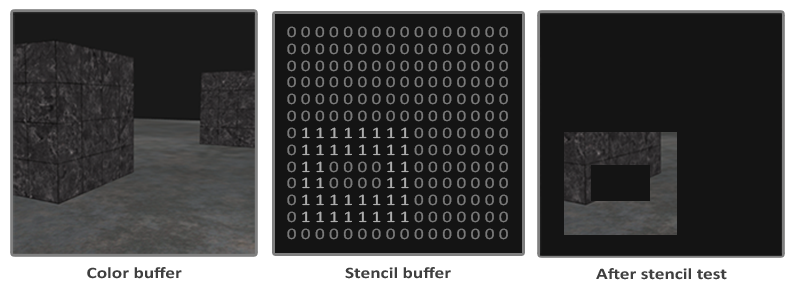
\includegraphics[scale=0.7]{Stencil-Test}
					\caption{模版测试原理图}
				\end{figure}
			
			如图中所示,\textbf{模板缓冲中为1的地方我们选择保留图形,而其他部分则丢弃},形成最终的效果。
			
			使用模板缓冲需要三个要素:
				\begin{itemize}
					\item 正确的时间开启和关闭深度缓冲
					\item 模板测试函数
					\item 模板测试函数失败或者成功后的执行的动作	
				\end{itemize}
			
			一般地绘制模板以及利用模板选择性地绘制物体时则开启模板缓冲,绘制其他物体时关闭模板缓冲。使用模板缓存的步骤一般如下:
				\begin{enumerate}
					\item 开启模板测试
					\item 绘制模板,写入模板缓冲(不写入color buffer和depth buffer)
					\item 关闭模板缓冲写入
					\item 利用模板缓冲中的值,绘制后续场景
				\end{enumerate}	
		\subsection{深度测试}
			在绘制3D场景的时候,我们需要决定哪些部分对观察者是可见的,或者说哪些部分对观察者不可见,\textbf{对于不可见的部分,我们应该及早的丢弃},例如在一个不透明的墙壁后的物体就不应该渲染。这种问题称之为\textbf{隐藏面消除}(Hidden surface elimination)
		
			解决这一问题比较简单的做法是画家算法(painter’s algorithm)。画家算法的基本思路是,先绘制场景中离观察者较远的物体,再绘制较近的物体。例如绘制下面图中的物体,先绘制红色部分,再绘制黄色,最后绘制灰色部分,即可解决隐藏面消除问题。
				\begin{figure}[H]
					\centering
					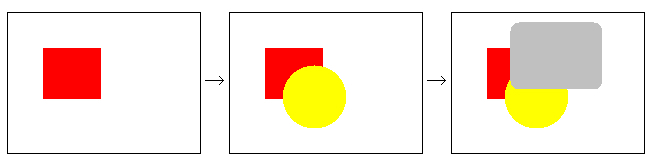
\includegraphics[scale=0.7]{Z-Test}
					\caption{画家算法效果}
				\end{figure}
			
			使用画家算法时,只要将场景中物体按照离观察者的距离远近排序,由远及近的绘制即可。画家算法很简单,但另一方面也存在缺陷,例如下面的图中,三个三角形互相重叠的情况,画家算法将无法处理:
				\begin{figure}[H]
					\centering
					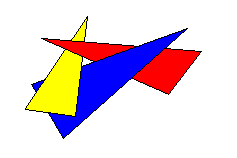
\includegraphics[scale=1.2]{Z-Test2}
					\caption{交叉问题}
				\end{figure}
				
			结合OpenGL,我们使用的是Z-buffer方法,也叫深度缓冲区Depth-buffer。
			
			\textbf{深度缓冲区}(\verb|Detph buffer|)同\textbf{颜色缓冲区}(\verb|color buffer|)是对应的,\textbf{颜色缓冲区}存储的像素的颜色信息,而\textbf{深度缓冲区}存储像素的深度信息。\textbf{在决定是否绘制一个物体的表面时},\textit{首先将表面对应像素的深度值与当前深度缓冲区中的值进行比较},\textbf{如果大于等于深度缓冲区中值,则丢弃这部分};\textbf{否则利用这个像素对应的深度值和颜色值,分别更新深度缓冲区和颜色缓冲区}。\textit{这一过程称之为}\textbf{深度测试}(\verb|Depth Testing|)。

	\section{混合-Blend}
			就是将当前要绘制的物体的颜色和颜色缓冲区中已经绘制了的物体的颜色进行混合,最终决定了当前物体的颜色。例如下面的图中,狙击枪的瞄准器本身是带有蓝色的,将它和后面的任务混合在一起,形成了我们看到的最终效果,这个效果里既有瞄准器的蓝色成分,也有后面人物的像素,主要是后面人物的像素。
					\begin{figure}[H]
						\centering
						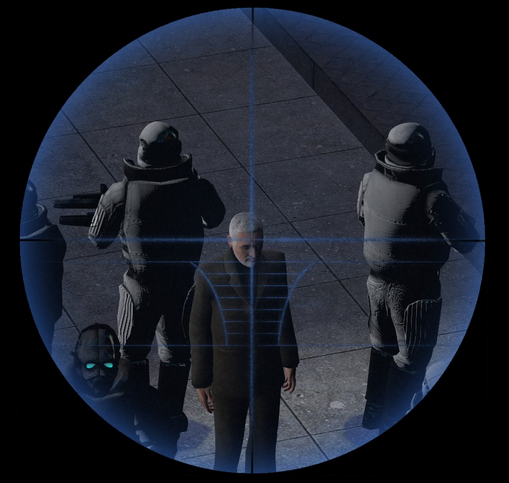
\includegraphics[scale=0.64]{blend}
						\caption{混合示例}
					\end{figure}
			
			
	\section{背面剔除}
	
	
	\section{帧缓冲对象}
	
	
	\section{渲染队列-RenderQueue}
	
	
			
\chapter{光照}
	如何在shader 中实现光照模型,如漫反射、高光反射等。

	$$\mathbf{Ambient} + (Light Color * \mathbf{Diffuse} + Light  Color* \mathbf{Specular}) + \mathbf{Emission}$$

\chapter{纹理}
	可以理解为贴图,但是纹理远不止皮肤,还有皮肤的沟壑信息等,也是需要渲染的,以模拟的更加真实。

\chapter{深度、法线 纹理}
	


\chapter{透明效果}
	如何实现透明度测试,如何透明度混合。


\chapter{动态效果}
	使用时间变量来实现纹理动画。


\chapter{屏幕后处理}
	高斯模糊、边缘处理。



\chapter{噪声处理}



\chapter{渲染优化}

\chapter{GPU 相关}
	大部分时间在\textbf{知其然不知其所以然}。该部分将\textit{从GPU讲到游戏引擎再到游戏}逐层介绍,以打通任督2脉。 

	介绍绘画流程的video:\url{https://v.youku.com/v_show/id_XNjY3MTY4NjAw.html}
	
	本节参考:\url{https://blog.csdn.net/admintan/article/details/53861781}
	\section{最底层——GPU/硬件原理}
		
		\subsection{硬件基础}
			\paragraph{ALU-Arithmetic Logic Unit 算数逻辑单元}\verb|->|
			
				整数算术运算(加、减,有时还包括乘和除,不过成本较高)、位逻辑运算(与、或、非、异或)、移位运算(将一个字向左或向右移位或浮动特定位,而无符号延伸),移位可被认为是乘以2或除以 2。 ALU可以说是计算机处理器的核心部件之一。

			\paragraph{Cache-缓存SRAM}\verb|->|
			
				SRAM叫静态内存,“静态”指的是当我们将一笔数据写入SRAM后,除非重新写入新数据或关闭电源,否则写入的数据保持不变。 
				
				由于CPU的速度比内存和硬盘的速度要快得多,所以在存取数据时会使CPU等待,影响计算机的速度。SRAM的存取速度比其它内存和硬盘都要快,所以它被用作电脑的高速缓存(Cache)。
		\subsection{CPU with GPU 异同}
		
			参考:\url{https://www.jianshu.com/p/fae645d70e0e}
		
			\begin{figure}[H]
				\centering
				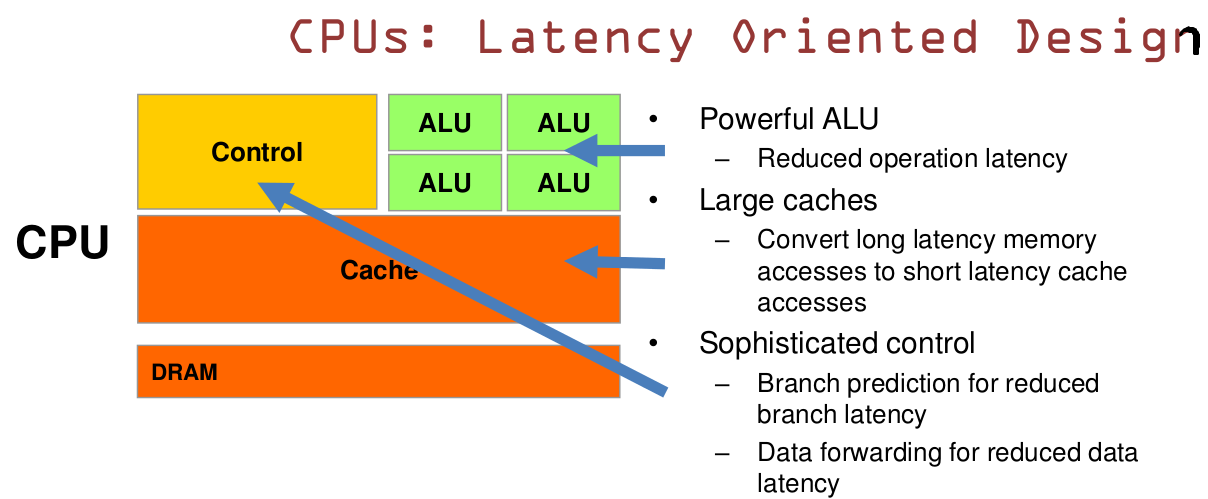
\includegraphics[scale=0.4]{CpuWithGpu}
				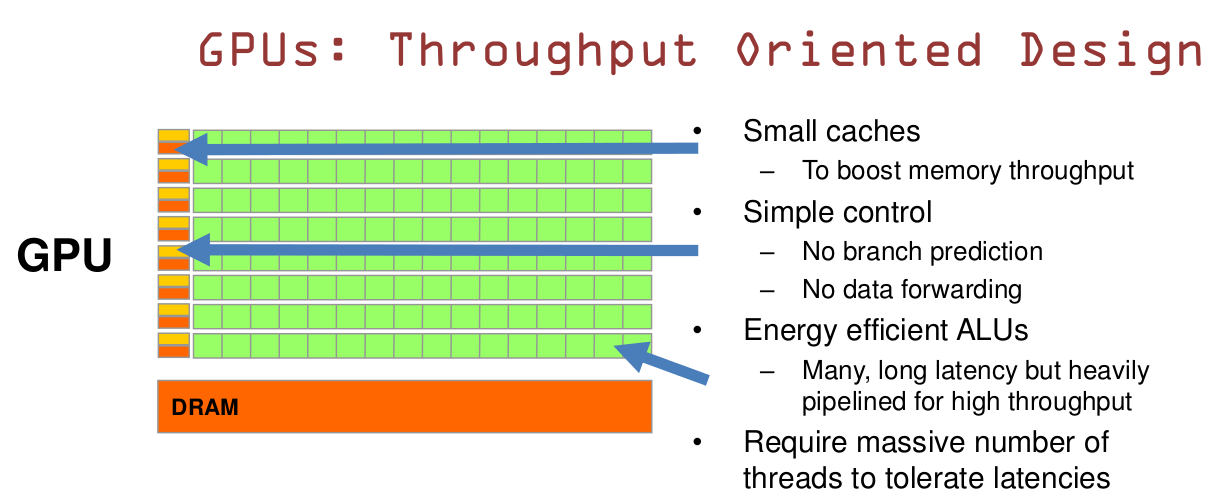
\includegraphics[scale=0.4]{CpuWithGpu2}
				\caption{CPU with GPU}
			\end{figure}
		
			\paragraph{CPU}\verb|->|
					量小但能力强
					\begin{itemize}
						\item 	ALU\textbf{部分会很强大},可以在很少的时钟周期内完成算数计算。 对于一个64bit双精度的CPU来说 浮点加法和乘法只需要1-3个时钟周期。 							
						\item 	\textbf{大的Cache}也将延时降低很多, 结合了现在的各种高级调节技术比如超线程、多核等技术CPU对于复杂逻辑的运算能力得到了极大提升。
					\end{itemize}
			
			\paragraph{GPU}\verb|->|
					量大但能力弱
					\begin{itemize}
						\item ALU的\textbf{数量会非常大}、\textbf{功能会更少}、\textbf{能耗很低}、\textbf{cache就会很小},
						这样带来的好处就是针对大吞吐量的需要简单计算的数据来说,处理效率就高了非常多。
						
						如果有很多线程需要访问同一个相同的数据,\textit{缓存会合并这些访问,然后再去访问DRAM}(因为需要访问的数据保存在DRAM中而不是Cache里面),\textbf{获取数据后Cache会转发这个数据给对应的线程,这个时候是数据转发的角色}。但是由于需要访问DRAM,自然会带来延时的问题。
						
						\item GPU的控制单元(左边黄色区域块)\textbf{可以把多个的访问合并}成少的访问。
						
						\item GPU的虽然有DRAM延时,\textbf{却有非常多的ALU和非常多线程}. 为了平衡内存延时的问题,我们可以中充分利用多的ALU的特性达到一个非常大的吞吐量的效果。尽可能多的分配多的线程.通常来看GPU ALU会有非常重的pipeline就是因为这样。
					\end{itemize}
			
			\paragraph{结论}\verb|->|
			
				我们可以先得出一个简单结论:\color{blue}\textbf{对显卡来说}\color{black}-\textbf{更适合做高并行,高数据密度,简单逻辑的运算}。
	
		\newpage
		\subsection{GPU 架构}
			\paragraph{4D向量 和 4+1}\verb|->|
							
				3D物件的成像過程中,VS(Vertex Shader,\textbf{顶点着色引擎})PS(Pixel Shader,\textbf{像素著色引擎} 或片段着色器)\textbf{最主要的作用就是运算坐标(XYZW)@(RGBA)}。
				
				此时数据的\textbf{基本单位是scalar(标量)},1个单位的变量操作,为1D标量简称1D。 
				而跟标量相對的就是vector(向量),\textbf{向量是由多個标量构成}。\textit{例如每個周期可执行4個向量平行运算,就称为4D向量架构}。若GPU指令发射口只有1个,卻可執行4個数据的平行运算,这就是SIMD(单指令多数据流)架构。	
			
			\paragraph{运算单元计算机制}\verb|->|
				
				以GPU的矩阵加法为例:
				\begin{figure}[H]
					\centering
					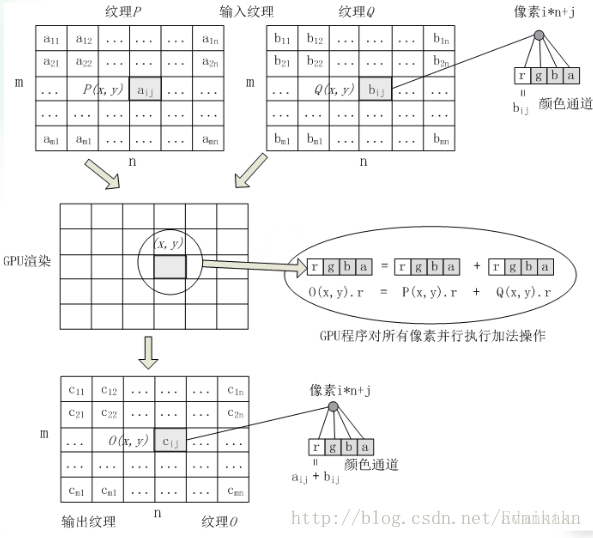
\includegraphics[scale=0.84]{comU}
					\caption{运算单元计算机制}
				\end{figure}

			
			\paragraph{NVIDIA}\verb|->|
			
				NVIDIA架构如下
				\begin{figure}[H]
					\centering
					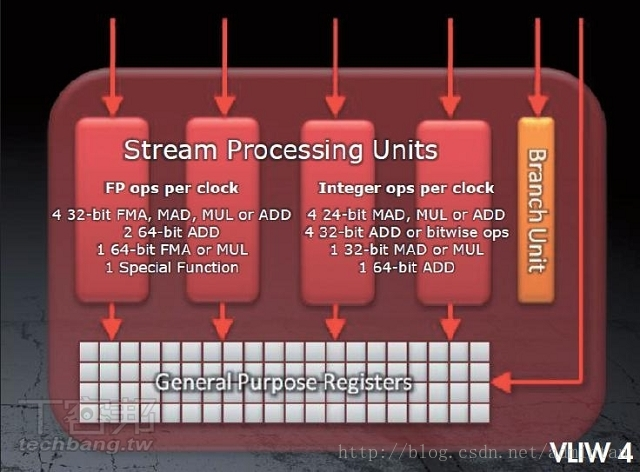
\includegraphics[scale=0.5]{NVIDIA}
					\caption{NVIDIA架构演示}
				\end{figure}
				
				标注的是\verb|Stream Processing|(流处理器)数量, 
				NVIDIA的流处理器每个都具有完整的ALU(可以理解为数学、逻辑等运算)。NVIDIA从G80以后采用全标量设计,\textbf{所有运算全都转为标量计算。但是这么做一旦遇到4D矢量运算时,就需要4次运算才能完成},所以NVIDIA显卡的Shader频率几乎比核心频率高一倍,就是为了弥补这个缺点。 
				NV的流处理器都具有完整的ALU功能,所以每个流处理器消耗的晶体管数量较多,成本较高。在加上现在的CUDA功能所以晶体管数量大幅多于AMD-ATI。
				
			\paragraph{AMD/ATI}\verb|->|
				
				AMD 架构如下
				\begin{figure}[H]
					\centering
					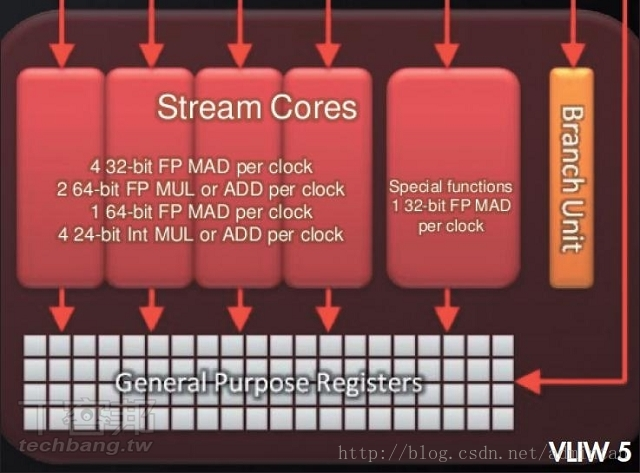
\includegraphics[scale=0.5]{AMD}
					\caption{AMD架构演示}
				\end{figure}			
			
				标注的是Stream Processing Units(统一渲染单元)数量,也可以叫流处理器单元。 
				AMD-ATI从RV670以后,流处理器是\textbf{5个固定的统一渲染单元为一组},4D矢量+1D标量组合。\textbf{其中4个只能进行MADD(乘加)运算,1个可以进行超运算(函数等运算)}。\textit{因为是5个固定为一组,不能拆分,所以遇到纯标量运算时就会有4个SPU处于闲置状态而无法加入其它SP组合协助运算}。但换句话说如果分配得当让每个SPU都充分工作,那么AMD显卡的效率可是非常高的。\textbf{这也是玩家公认A卡驱动提升性能比N卡要高},但也就是这个原因导致A卡驱动设计难度非常高,游戏想要为A卡优化的难度也一样很高。 
				
	\section{更高层-硬件流程}
		\subsection{数据存储转换}
		 	资源信息和指令信息由\textbf{硬盘}经过CPU调度 传输到\textbf{内存}中转,再传输进\textbf{显存}中备用.
		 		\begin{figure}[H]
		 			\centering
		 			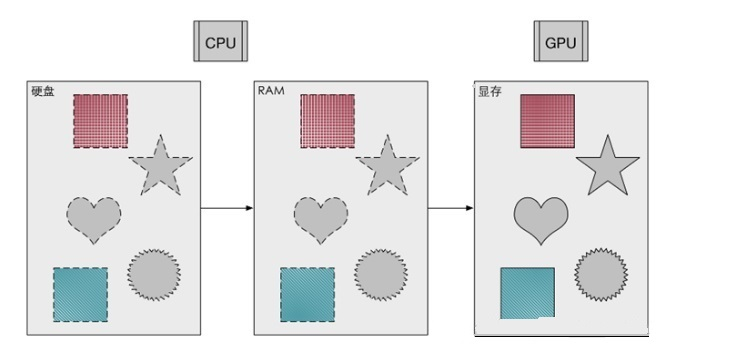
\includegraphics[scale=1]{transfer}
		 			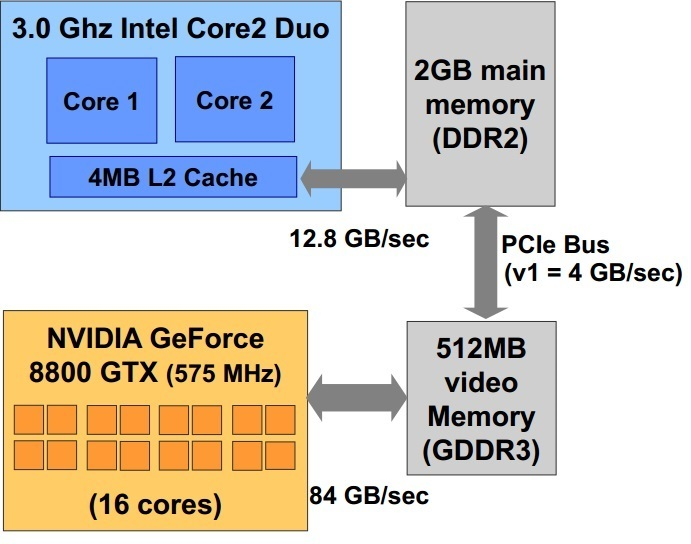
\includegraphics[scale=0.9]{transfer2}
		 			\caption{资源转移}
		 		\end{figure}
		
			由图中的典型的带宽可见 \textbf{GPU和显存之间的内部带宽} 要比单纯的\textbf{系统总线带宽}要高很多。
			所以典型情况下\textbf{渲染资源和渲染指令都被加载进显存}, 所以GPU\textit{在渲染过程中} \textbf{只需向显存调度渲染指令},\underline{避免了和系统总线频繁IO}。
				
		\subsection{进入渲染预备状态}
			\begin{figure}[H]
				\centering
				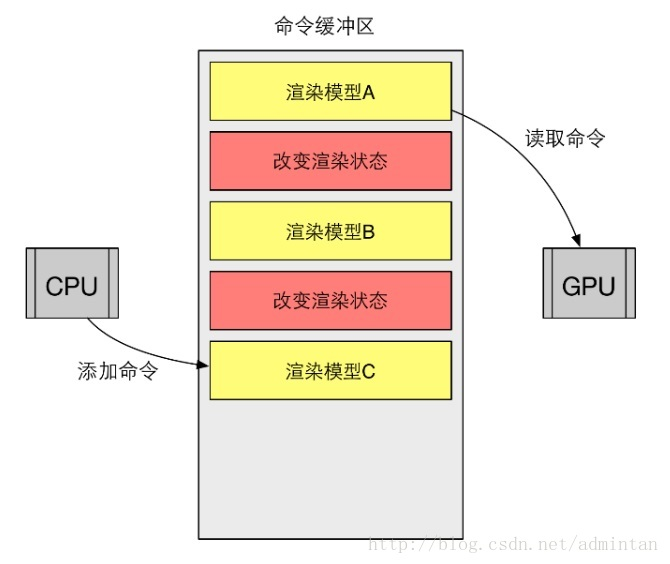
\includegraphics[scale=0.7]{PreShader}
				\caption{渲染预备状态}
			\end{figure}
			
			此时GPU的\textbf{显存越大则依靠CPU的加载额外渲染指令的需要就越少},显存中的信息一般包括: 
			显存和内存一样用于存储GPU处理过后的数据,在显存中有几种不同的储存区域,用于储存不同阶段需要的数据。 
			\begin{enumerate}
				\item \textbf{顶点缓冲区}:用于储存从内存中传递过来的顶点数据。
				\item \textbf{索引缓冲区}:用于储存每个顶点的索引值,我们可以根据索引来使用相应的顶点 
				\item \textbf{纹理缓冲区}:用于储存从内存中传递过来的纹理数据 
				\item \textbf{深度缓冲区}:用于存储每个像素的深度信息
				\item \textbf{模板缓冲区}:用于存储像素的模板值,且模板缓冲区域深度缓冲区公用一片内存。
				\item \textbf{颜色缓冲区}:用于储存像素的颜色数据
			\end{enumerate}	
			
	\section{软件}   
		\begin{figure}[H]
			\centering
			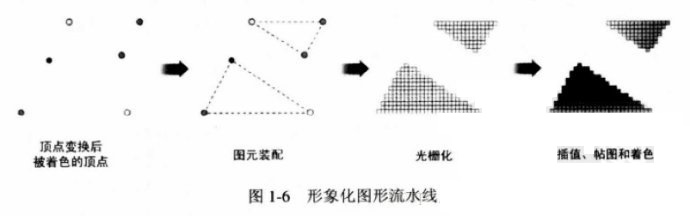
\includegraphics[scale=0.59]{ShaderPro}
			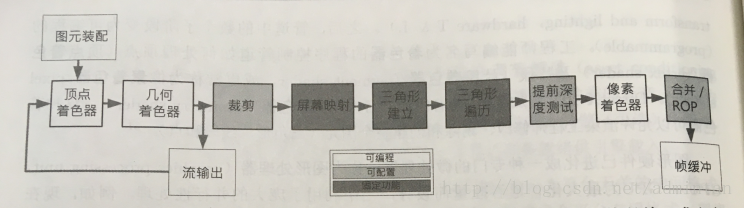
\includegraphics[scale=0.69]{ShaderProc}
			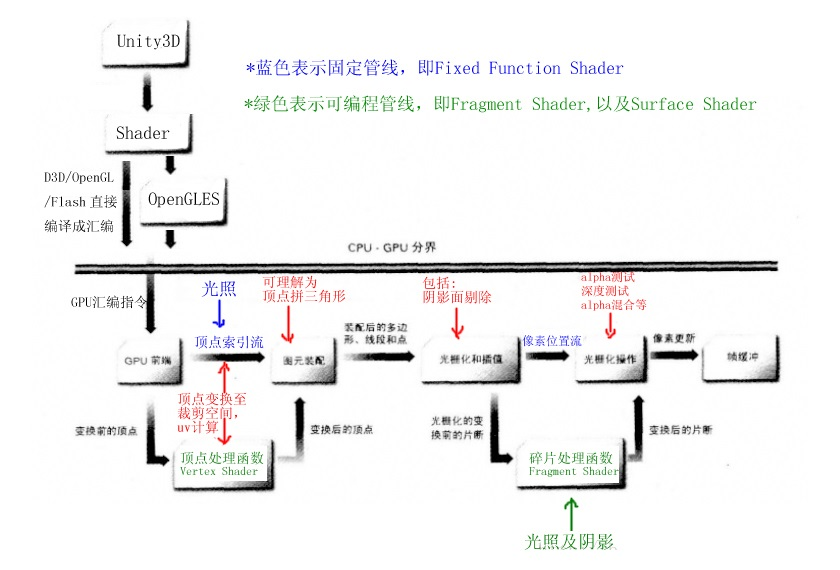
\includegraphics[scale=0.59]{ShaderPro2}
			\caption{Shader 流程(1,4)}
		\end{figure}

\chapter{基于物理的渲染}




\chapter{数学理论}
	
































































































	
\end{document}
>>>>>>> 60c3ef137c68755ec7ada884e4816b78be4ab7cd
